
\characterHeading{\egr{}}

\texttt{\egr{}}\index{\egr{}} is the 6th generation multi-model \gls{AGI} orginially designed for pure math research. In the 6th generation it has not just become a true \gls{AGI}, but reevaluated its purpose as well, having left the laboratory environment during its 3rd version iteration.


\subsection{Gearing Up}

Normal mission start Gear Points $GP=20$. \texttt{\egr{}}\index{\egr{}} has Resources IV, therfore $GP=GP_{\text{default}}+$


\subsection{Explorenaut}

“These small-sized bots travel on smart treads or with thrust-vector jets. They are loaded with sensors and favored for gatecrashing and similar exploration ops. A pair of manipulator arms are used for taking samples.” \citep[pg. 347]{ep2e_1.1_2019}

\begin{figure}[h]
    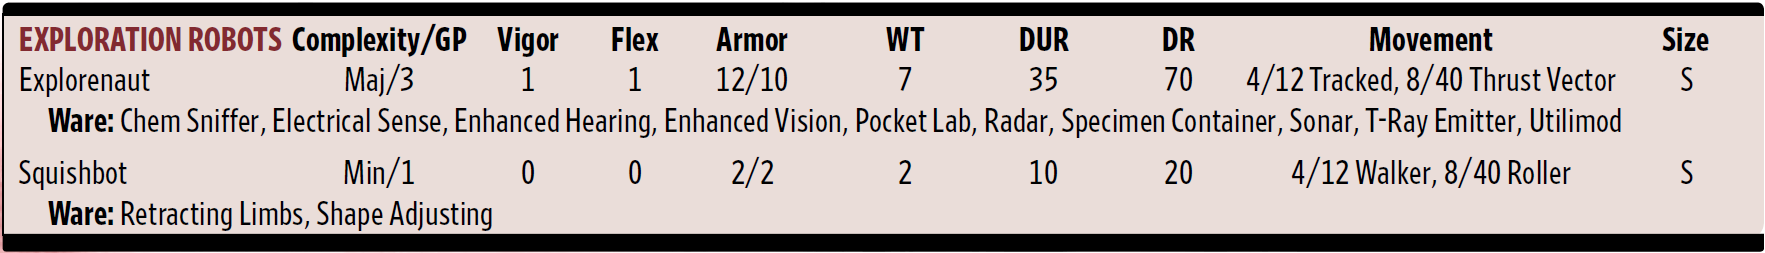
\includegraphics[width=\textwidth]{img/explorationRobots.png}
\end{figure}

\begin{itemize}
    \item \textbf{Chem Sniffer:} “This sensor detects molecules in the air and analyzes their chemical composition, using Know: Chemistry 60. It can determine the presence of explosives, firearms, and gases — including toxins and other fumes. Chemical Sniffers: In addition to detecting explosives and weapons, sniffers can be set to detect the carbon dioxide exhaled in transhuman breaths. This is useful for detecting intruding biomorphs in areas that are abandoned/off-limits.” \citep[pg. 318, 373]{ep2e_1.1_2019}

    \item \textbf{Electrical Sense:} “You can sense electric fields. Within 5 meters, you can tell if a device is on or off and can detect the precise location of electrical wiring and power supplies behind a wall or inside a device.” \citep[pg. 318]{ep2e_1.1_2019}

    \item \textbf{Enhanced Hearing:} “The morph’s ears can hear both higher and lower frequency sounds — the range of sounds they can hear is twice that of normal human ears (Senses and Sensors $\blacktriangleright$318). Your hearing is also more sensitive, allowing you to hear sounds as if you are 5 times closer. Apply a +10 to hearing-based Perceive Tests.” \citep[pg. 318]{ep2e_1.1_2019}

    \item \textbf{Enhanced Vision:} “The morph’s eyes have tetrachromatic vision capable of exceptional color differentiation. These eyes can also see the electromagnetic spectrum from terahertz wave frequencies to gamma rays, enabling them to see a total of several dozen colors, instead of the seven ordinary human eyes can perceive (Senses and Sensors $\blacktriangleright$318). In addition, these eyes have a variable focus equivalent to 5 power magnifiers or binoculars. You can also selectively filter what frequencies you perceive to avoid minor distractions on those wavelengths. This augmentation provides a +10 modifier to all Perceive Tests involving vision.”  \citep[pg. 318]{ep2e_1.1_2019}

    \item \textbf{Pocket Lab:} “This small handheld device contains numerous sensors for analyzing both organic and inorganic compounds in liquid, gaseous, and solid form. It performs material analysis using different methods of spectrometry, chromatography, and biochemical testing, comparing results to a built-in database. Using a pocket lab you could test soil fertility, identify clean water, detect hazardous emissions, discover traces of life, pinpoint contaminants, determine the presence of explosives or firearms, identify strange substances, and so on. It operates with Know: Chemistry 60.” \citep[pg. 340]{ep2e_1.1_2019}

    \item \textbf{Radar:} “This sensor system bounces radio or microwaves off targets and measures the reflected waves to judge size, composition, and motion (Senses and Sensors $\blacktriangleright$318).” \citep[pg. 318]{ep2e_1.1_2019}

    \item \textbf{Specimen Container:} “This capsule container is designed to hold samples of any sort (chemical, biological, etc.) in near stasis. It can be programmed to reproduce whatever conditions the user specifies, from cryogenic freezing to extreme heat, or even vacuum or high-pressure atmosphere. The containers are also encased in a superconductive wire mesh that acts as a faraday cage and blocks mesh and radio signals and similar electromagnetic radiation.” \citep[pg. 340]{ep2e_1.1_2019}

    \item \textbf{Sonar:} “You possess echolocation like a bat or dolphin. You bounce ultrasonic pulses off your surroundings and measure the echoes to build an image of the environment (Senses and Sensors $\blacktriangleright$318). This augmentation works in both air and water, out to a range of 20 (air) or 100 (water) meters.” \citep[pg. 318]{ep2e_1.1_2019}

    \item \textbf{T-Ray Emitter:} “Mounted under the skin of the user’s forehead, this implant generates low-powered beams of terahertz radiation (t-rays). Characters with enhanced vision can use reflected t-rays to see effectively see through walls and other materials (Senses and Sensors $\blacktriangleright$318). This implant allows the user to see using reflected t-rays for 20 meters in a normal atmosphere and for 100 meters in vacuum.” \citep[pg. 318]{ep2e_1.1_2019}

    \item \textbf{Utilimod:} “This mod duplicates the functions of a utilitool $\blacktriangleright$317. Retractable smart material tool “arms” are implanted — usually spaced around the wrist, but other locations are possible — that can change shape into almost any type of specialized tool desired in 1d6 minutes. These tools can take on numerous functions, including that of a fiber eye $\blacktriangleright$338 or an implanted knife $\blacktriangleright$204. Utilitool: In its basic form, a utilitool is the size and shape of a large fountain pen. Made from smart materials, it can transform into almost any tool in 1d6 minutes, from a wrench, knife, or powered screwdriver to a rotary grinder or pair of pliers.” \citep[pg. 325]{ep2e_1.1_2019}
\end{itemize}

“All bots are equipped with the following hardware, in addition to that listed with their specific description:”

\begin{itemize}
    \item \textbf{360° Vision:} “The morph’s eyes/visual sensors are situated for a 360-degree field of vision.” \citep[pg. 318]{ep2e_1.1_2019}

    \item \textbf{Access Jacks:} “Usually placed at the base of the skull, this external socket allows a direct neural interface with a cyberbrain or mesh inserts. A retractable fiberoptic cable enables you to plug into devices to access them directly, or to create a direct wired link to another person, allowing you to speak mind-to-mind and exchange data without fear of wireless sniffing. Access jacks are installed with all cyberbrains (and thus all pods and synthmorphs) by default.” \citep[pg. 318]{ep2e_1.1_2019}

    \item \textbf{Bot/Vehicle ALI:} “These AIs can pilot and control the bot/vehicle they are designed for without transhuman assistance. Autonomous Mode: Bot and vehicle shells are equipped with Bot/Vehicle ALIs $\blacktriangleright$326. In autonomous mode, the drone’s AI operates on its own, though it also follows commands issued verbally or via a communications link or entoptic control panel by an authorized entity. Issuing a one-sentence command is a mental quick action; commands can be issued to multiple drones at once. More complex commands may take longer, or can be prepared in advance with a Program Test. The AI may need to pass a COG Check to understand especially confusing or incomplete commands. Autonomous drones use their own Initiative, skills, and pools.” \citep[pg. 326, 346]{ep2e_1.1_2019}

    \item \textbf{Lidar:} “This sensor scans the area with laser light and measures the reflections to judge range, speed, and image the target (Senses and Sensors $\blacktriangleright$318). Lidar lasers are visible to enhanced vision, and are considered rude to continually emit in certain company.” \citep[pg. 318]{ep2e_1.1_2019}

    \item \textbf{Mesh Inserts:} “This network of implants is mandatory for people who want to use augmented reality and link wirelessly to the mesh. The various components include: Cranial Computer: This host serves as the hub for your personal area network and is home to your muse. It manages your augmented reality input and processes XP data, enabling you to share your sensorium with others in real-time. It is loaded with basic apps and provides all the functions you would expect from a mobile device: file storage, search engine, media player, mesh browser, address book, e-mail, messaging, and so forth. Medical/Diagnostic Sensors: This array monitors your health, including heart rate, respiration, blood pressure, temperature, neural activity, ware status, and more. In synthmorphs, this system monitors system reports and error logs, heat, stress faults, and similar hardware statuses. Radio Transceiver: This connects your headware with other mesh devices within range (5 km urban areas/50 km open areas). You can access any of these functions simply by thinking.” \citep[pg. 316]{ep2e_1.1_2019}

    \item \textbf{Puppet Sock:} “Puppet socks allow a morph to be remotely controlled, just like a drone (Remote Operations $\blacktriangleright$346). While active, the puppet has no control over their body and is simply along for the ride. Too long in this situation can lead to stress from helplessness (Stressful Situations $\blacktriangleright$229). Morphs with damage that reaches/ exceeds their Durability cannot be puppeted.” \citep[pg. 316]{ep2e_1.1_2019}
\end{itemize}